\documentclass[a4paper,11pt]{article}

\usepackage[utf8]{inputenc}

\usepackage{minted}
\usepackage{graphicx}

\begin{document}


\title{
    \textbf{Stack report}
}
\author{Jonathan Karlsson}
\date{Fall 2023}

\maketitle

\section*{Introduction}

The assignment involved creating a stack for an RPN calculator. The calculator was to be made with two different types of stack, 
a dynamic stack and a static stack. The dynamic stack is able to grow and shrink depending on its use while the static stack can only
use the amount dedicated to it when it was created. The report will describe the differences between the stacks and also benchmark them.

\section*{Implementation}

The stack was implemented as a static stack and a dynamic stack, where the static stack has a 
specified size and the dynamic stack can change the size if the stack is too small.
Both stacks have similar pop and push methods, however there are some differences in these methods, explained later.


\subsection*{Static stack}
The static stack was implemented such that the size of the stack is selected when the stack is created.
\begin{minted}{java}
    public StaticStack(int size) {
        this.size = size;
        stack = new int[size];
}
\end{minted}
The size is dependent on how many operations are needed and therefore how many numbers are stored in the
stack. The push method has a check incase the size of the stack is too samll for the data in it.
This occurs when the stack pointer is at the end of the stack but there is still data that is supposed to 
be pushed onto the stack. The pop method also has a check to see if the pointer is at the start of the stack
when data is supposed to be popped from the stack. If the checks fail when pushing or popping a StackExcpetion is thrown.
\begin{minted}{java}
public void push(int value){
    
    if (pointer >= this.size)
        throw new StackException("Stack too small");
    stack[pointer] = value;
    pointer++;
}    
public int pop(){
if (pointer > 0) {
    pointer--;
    return stack[pointer];
}
else 
    throw new StackException("Stack is empty, check input");

}  
\end{minted}

\subsection*{Dynamic stack}

The dynamic stack was implemented using similar code to the static stack.
The constructor for the dynamic stack was different from the static stack as it has 
a default value for the size or a settable size. If the size is manually set the 
stack will start to shrink once the pointer is over 1/4 of the total size of the stack
and has started decreasing.
\begin{minted}{java}
public DynamicStack(int size) {
    this.size = size;
    stack = new int[this.size];
    pointer = 0;
}

public DynamicStack() {
    this(4);
    
}  
\end{minted}
The push and pop methods in the dynamic stack were both changed. The push method was changed such that when the stack overflows, instead
of throwing a StackException the stack is instead expanding using the increaseSize method. The pop was also changed so that
the stack shrinks using the decreaseSize method whenever the pointer has gone down to 1/4 of the total size of the stack.
This is implemented so that the stack will not keep increasing and decreasing in size every push and pop
as the stack increases with 2 times itself, it waits until it has reached 1/4 of use before decreasing by half.
\begin{minted}{java}
public void push(int value){
    
    if (pointer >= size)
        increaseSize();
    stack[pointer] = value;
    pointer++;
}    
public int pop(){

if (pointer > 0) {
    pointer--;
    if (size/(pointer+1) == 4)
        decreaseSize(); 
    return stack[pointer];
}
else 
    throw new StackException("Stack is empty, check input");

}
\end{minted}
\subsubsection*{IncreaseSize and decreaseSize}
The increaseSize method is a simple copy algorithm which first copies the entire array into an
array that is twice the size and then sets the first array equals to the new array.
The decreaseSize method works in a similar way except for the fact that the decreaseSize
method halves the size of the stack instead of doubling it.
\begin{minted}{java}
private void increaseSize() {

size *= 2; 
int[] newStack = new int[size];
int index = 0;
for (int copyItem : stack){
    newStack[index] = copyItem;
    index++;
}
stack = newStack;
}

private void decreaseSize() {

size /= 2;
int[] newStack = new int[size];
for (int index = 0; index < size; index++){
    newStack[index] = stack[index];
}
stack = newStack;
}
  
\end{minted}



\section*{Benchmark}
The benchmark for the stacks involved first pushing a set amount of elements onto the stack and
then popping them immediately afterwards. This was done a total of 1000 times for each set of elements
and each stack and then the minimum time of the runs was saved for that particular set of elements on that stack.
\subsection*{Results}
The results of the benchmark looked promising as the time the dynamic stack took went down in relation to the static stack.
This is becuase the stack doubles in size by 2 each time it runs out of space. This means that it 
is able to stay at the same size for longer as the size increases. The result is in microseconds and with one 
decimal place.
\subsubsection*{}
\begin{table}[h]
    \begin{center}
    \begin{tabular}{l|c|c|c}
    \textbf{n} & \textbf{static ({\textmu}s)} & \textbf{dynamic ({\textmu}s)} &\textbf{ratio (d/s)}\\
    \hline
    25   &    0.1 &    2.6 &   26.0\\
    50   &    0.3 &    2.8 &   9.3\\
    100  &    0.4 &    3.3 &   8.2\\
    250  &    0.6 &    4.3 &   7.1\\
    500  &    1.2 &    5.6 &   4.7\\
    1000 &    2.3 &    8.3 &   3.6\\

    \end{tabular}
    \caption{The results of the benchmark for the different stacks}
    \label{tab:table1}
    \end{center}
\end{table}
\subsubsection*{}
Using a graph it is possible to visualise how the times of the two stacks develops. 
The graph shows that both stacks have a linear kind of development, however the first 
set of elements of the dynamic stack takes longer, and the dynamic stack also increases more per
element.

\begin{figure}[h]
\centering    

\scalebox{0.5}{% GNUPLOT: LaTeX picture with Postscript
\begingroup
  % Encoding inside the plot.  In the header of your document, this encoding
  % should to defined, e.g., by using
  % \usepackage[cp1252,<other encodings>]{inputenc}
  \inputencoding{cp1252}%
  \makeatletter
  \providecommand\color[2][]{%
    \GenericError{(gnuplot) \space\space\space\@spaces}{%
      Package color not loaded in conjunction with
      terminal option `colourtext'%
    }{See the gnuplot documentation for explanation.%
    }{Either use 'blacktext' in gnuplot or load the package
      color.sty in LaTeX.}%
    \renewcommand\color[2][]{}%
  }%
  \providecommand\includegraphics[2][]{%
    \GenericError{(gnuplot) \space\space\space\@spaces}{%
      Package graphicx or graphics not loaded%
    }{See the gnuplot documentation for explanation.%
    }{The gnuplot epslatex terminal needs graphicx.sty or graphics.sty.}%
    \renewcommand\includegraphics[2][]{}%
  }%
  \providecommand\rotatebox[2]{#2}%
  \@ifundefined{ifGPcolor}{%
    \newif\ifGPcolor
    \GPcolortrue
  }{}%
  \@ifundefined{ifGPblacktext}{%
    \newif\ifGPblacktext
    \GPblacktextfalse
  }{}%
  % define a \g@addto@macro without @ in the name:
  \let\gplgaddtomacro\g@addto@macro
  % define empty templates for all commands taking text:
  \gdef\gplbacktext{}%
  \gdef\gplfronttext{}%
  \makeatother
  \ifGPblacktext
    % no textcolor at all
    \def\colorrgb#1{}%
    \def\colorgray#1{}%
  \else
    % gray or color?
    \ifGPcolor
      \def\colorrgb#1{\color[rgb]{#1}}%
      \def\colorgray#1{\color[gray]{#1}}%
      \expandafter\def\csname LTw\endcsname{\color{white}}%
      \expandafter\def\csname LTb\endcsname{\color{black}}%
      \expandafter\def\csname LTa\endcsname{\color{black}}%
      \expandafter\def\csname LT0\endcsname{\color[rgb]{1,0,0}}%
      \expandafter\def\csname LT1\endcsname{\color[rgb]{0,1,0}}%
      \expandafter\def\csname LT2\endcsname{\color[rgb]{0,0,1}}%
      \expandafter\def\csname LT3\endcsname{\color[rgb]{1,0,1}}%
      \expandafter\def\csname LT4\endcsname{\color[rgb]{0,1,1}}%
      \expandafter\def\csname LT5\endcsname{\color[rgb]{1,1,0}}%
      \expandafter\def\csname LT6\endcsname{\color[rgb]{0,0,0}}%
      \expandafter\def\csname LT7\endcsname{\color[rgb]{1,0.3,0}}%
      \expandafter\def\csname LT8\endcsname{\color[rgb]{0.5,0.5,0.5}}%
    \else
      % gray
      \def\colorrgb#1{\color{black}}%
      \def\colorgray#1{\color[gray]{#1}}%
      \expandafter\def\csname LTw\endcsname{\color{white}}%
      \expandafter\def\csname LTb\endcsname{\color{black}}%
      \expandafter\def\csname LTa\endcsname{\color{black}}%
      \expandafter\def\csname LT0\endcsname{\color{black}}%
      \expandafter\def\csname LT1\endcsname{\color{black}}%
      \expandafter\def\csname LT2\endcsname{\color{black}}%
      \expandafter\def\csname LT3\endcsname{\color{black}}%
      \expandafter\def\csname LT4\endcsname{\color{black}}%
      \expandafter\def\csname LT5\endcsname{\color{black}}%
      \expandafter\def\csname LT6\endcsname{\color{black}}%
      \expandafter\def\csname LT7\endcsname{\color{black}}%
      \expandafter\def\csname LT8\endcsname{\color{black}}%
    \fi
  \fi
    \setlength{\unitlength}{0.0500bp}%
    \ifx\gptboxheight\undefined%
      \newlength{\gptboxheight}%
      \newlength{\gptboxwidth}%
      \newsavebox{\gptboxtext}%
    \fi%
    \setlength{\fboxrule}{0.5pt}%
    \setlength{\fboxsep}{1pt}%
    \definecolor{tbcol}{rgb}{1,1,1}%
\begin{picture}(7200.00,5040.00)%
    \gplgaddtomacro\gplbacktext{%
      \csname LTb\endcsname%%
      \put(330,440){\makebox(0,0)[r]{\strut{}$0$}}%
      \put(330,927){\makebox(0,0)[r]{\strut{}$1$}}%
      \put(330,1413){\makebox(0,0)[r]{\strut{}$2$}}%
      \put(330,1900){\makebox(0,0)[r]{\strut{}$3$}}%
      \put(330,2386){\makebox(0,0)[r]{\strut{}$4$}}%
      \put(330,2873){\makebox(0,0)[r]{\strut{}$5$}}%
      \put(330,3359){\makebox(0,0)[r]{\strut{}$6$}}%
      \put(330,3846){\makebox(0,0)[r]{\strut{}$7$}}%
      \put(330,4332){\makebox(0,0)[r]{\strut{}$8$}}%
      \put(330,4819){\makebox(0,0)[r]{\strut{}$9$}}%
      \put(462,220){\makebox(0,0){\strut{}$0$}}%
      \put(1096,220){\makebox(0,0){\strut{}$100$}}%
      \put(1730,220){\makebox(0,0){\strut{}$200$}}%
      \put(2364,220){\makebox(0,0){\strut{}$300$}}%
      \put(2998,220){\makebox(0,0){\strut{}$400$}}%
      \put(3633,220){\makebox(0,0){\strut{}$500$}}%
      \put(4267,220){\makebox(0,0){\strut{}$600$}}%
      \put(4901,220){\makebox(0,0){\strut{}$700$}}%
      \put(5535,220){\makebox(0,0){\strut{}$800$}}%
      \put(6169,220){\makebox(0,0){\strut{}$900$}}%
      \put(6803,220){\makebox(0,0){\strut{}$1000$}}%
    }%
    \gplgaddtomacro\gplfronttext{%
      \csname LTb\endcsname%%
      \put(5816,4646){\makebox(0,0)[r]{\strut{}static}}%
      \csname LTb\endcsname%%
      \put(5816,4426){\makebox(0,0)[r]{\strut{}dynamic}}%
    }%
    \gplbacktext
    \put(0,0){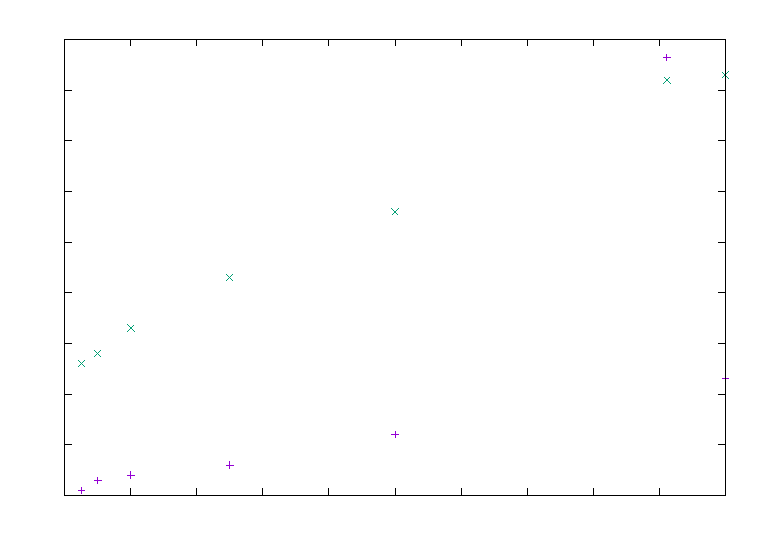
\includegraphics[width={360.00bp},height={252.00bp}]{disp}}%
    \gplfronttext
  \end{picture}%
\endgroup
}
\caption{Visualization of the times for the two diffent stacks}   
\label{tab:figure1} 

\end{figure}


\section*{Conclusion}
It seems that the different types of stacks are useful depending on the application. Incase the 
application requires that the stack is as fast as possible but does not care about the memory usage,
a static stack is best, however it could become problematic if the data turns out to be larger than the allocated stack, 
as the static stack does not allow increasing of the size. The dynamic stack is however more useful if the stack is allowed 
to take more time as the dynamic stack does not require a specific allocated amout. It is also more memory efficient as the stack 
decreases its own size whenever it has too much unused space.

\end{document}
